\chapter{Design and Methodology}

\label{Chapter3}

\lhead{Chapter 3. \emph{Design and Methodology}}

This chapter is about the blueprint and the Methodologies used in the thesis involves a systematic progression of 
the steps to ensure a careful exploration of the topic modelling techniques. The process contains various steps and the implementation 
will start from the point of data collection and then analysing the data leading to the interpretation of results and their 
alignment with the initial research objective. The collected data is analysed then transformed into a format that is conductive
for the effective processing which involves few steps like removal of unwanted data, combining the data, cleaning the data, and 
so on then, the data is used to feed into the model to obtain the results. Finally, the thesis concludes with a discussion
of findings, implications, and potential avenues for future research, presenting a well-rounded culmination of the research endeavour.
Figure 3.1 shows the implementation steps. These steps will be explained further below,

\begin{figure}[htbp]
    \begin{center}
      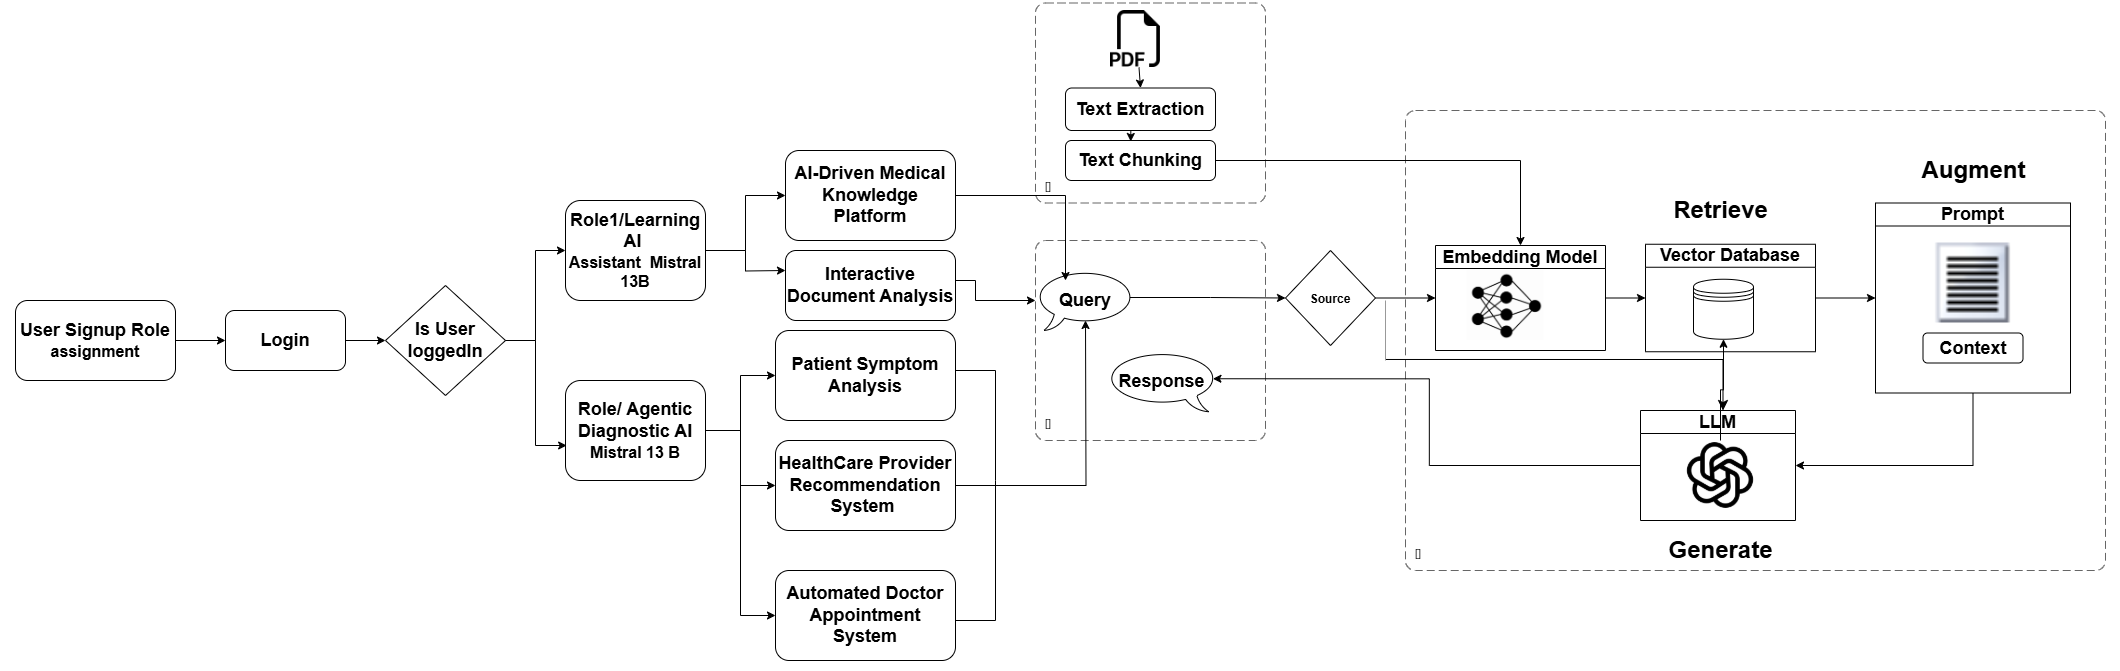
\includegraphics[width=15cm]{./Images/Thesis.png}
       \caption{Thesis implementation phases}
       \label{fig: Thesis implementation phases}
    \end{center}
    \end{figure}
% ============================================================================
% section : Data Collection and Analysis
% =============================================================================
\section{Data Collection and Analysis}

The data for this thesis is taken from the Fern Universität in Hagen, Germany. From the early 1980s to the present, 
Fern University has conducted numerous interviews as part of its contemporary history research projects. These include 
biographical interviews were individuals interviewees narrate their own stories and also gives their point of view on 
the events that occurred during that time. Apart from these biographical interviews, autobiographies, written texts and 
various letters are also collected from many people with different culture background but have a connection to social events 
in Germany. The video interviews are also present which has wide information about various topics like work councils, trade 
unionists, migrants, concentration camp survivors, and so on. The interviews contain some information
about the Germany history. There are about 350 Video interviews as part of the research which are convert into transcripts. 
The transcript of this dataset and contains three columns:

\begin{enumerate}
    \item\textbf{Timecode:} As the video interview is convert into transcript, the timecode is used to identify the 
    start and end of the interview. It is in the format of $hh:mm:ss$.
    \item\textbf{Sprecher:}  The name of the speaker in the interview.
    \item\textbf{Transcript:}  The interview transcript the conversation between the speakers.
\end{enumerate}
% ============================================================================
% section : Data Preprocessing
% =============================================================================
\section{Data Preprocessing}

Once the data is analysed it needs be Pre-processed in order to use it as the data might have mistaken, redundancies, 
missing values, or inconsistencies due to all these reasons it needs to be cleaned so that, we will be able to use it for 
further analysis. For example, during the training of a machine learning model it is important to clean the data in order 
to avoid overfitting or underfitting or wrong predictions. Hence, before using the dataset to any tasks it is better do some 
data cleaning if needed. There is not much Preprocessing is used in the thesis, but it is important to clean the data before 
using it. Few steps are followed in this thesis is mentioned below,

\begin{enumerate}
    \item\textbf{Removal of Unwanted columns}
    
    As the dataset has three columns of data, the timecode, the Sprecher and the transcript. In the Timecode column except 
    the timestamp of the video we don't have any information which can be used for analysis. Hence, it is removed.
    Sprecher column is removed as it is not required for the analysis. Since, it consists of the who speak that particular 
    sentence in the conversation and after analysis for the few transcripts it was not making much sense. Hence, it is removed.
    Transcript column is the key column which contains the main information of the conversation which is required for the analysis. 
    Here, the rows of the interviewer is not removed as may  contains the information which might be essential for the thesis.

    \item\textbf{Combining the data}
    
    As the dataset was in the excel format and each conversation transcript was in the form of a new line in the column 
    Transcript, it was necessary to combine the data into one single corpus. Hence, it is necessary to combine the data into 
    one a paragraph so that contexts of the conversation can be maintained, and which will help in the future phases. 
    On the other hand, the video conversation of each individual was available in the separate sheets in the excel file. 
    Hence, it is necessary to merge the data into a single text document. As the looping through each page and combining 
    them into a paragraph will take more time than the combination of the whole data. So, combining the data in one document
    will help to reduce the time taken for the analysis.

    \item\textbf{Removing the short sentences}
    
    As the transcript column was combined into a paragraph and there we have lot of sentences which are smaller than 3 words.
     This Sentence will act as nosie as there are repeated words, Stopwords, punctuations, etc. have formed the sentence which 
     is doesn't add value to the analysis as it is act like a noise in the data. Hence, it is necessary to remove all the sentences 
     that are smaller than 3 words. As it doesn't make sense to have a sentence with less than 3 words. So, filtered the short 
     sentences out of the dataset was done as it was like a noise in the data.

\end{enumerate}

There are few other steps that can be done to clean the data like Stopwords, punctuations, lemmatization, etc., which I haven't 
considered as it is not required. Since, these preprocessing is only required when we are doing word embedding hence, I have not 
considered it in the thesis. As I'll will doing sentence embedding which will help to capture the meaning of the sentences in 
the paragraph and get better results.
% ============================================================================
% section : Modelling
% =============================================================================


\section{Modelling}
In this stage, the approach of achieve topic modelling will be eaxplained. As the Preprocessing of the dataset is done. 
The dataset is ready for topic modelling where it will undergoes stages like embedding,
 dimensional reduction, clustering and generating the topic name using the language model. The various stages and mentioned 
 modelling techniques are explained by,
 \begin{figure}[htbp]
    \begin{center}
      \includegraphics[width=16cm]{./Images/Modelling Workflow.png}
       \caption{Modelling Workflow}
       \label{fig: Modelling Workflow}
    \end{center}
    \end{figure}
% ============================================================================
% subsection : Sentence Embedding
% =============================================================================
\subsection{Sentence Embedding}

After the Preprocessing of the dataset is done. The dataset is ready for embedding and as Sentence Embedding approach will 
be used to get the numerical representation of the text data which will help the machine learning model to understand the text data.
As the dataset is in German language choosing the good sentence embedding model is important to get better result as most of the 
embedding model are mostly trained on the English language Primary and then there are few models which are trained on multiple 
languages. So, choosing the good model is important to get better results. So, after careful examine some of the model for 
German language and few of the model is mentioned below,

 \begin{enumerate}
    \item GBERT Derived Embedding Models
    \item Sentence-T5 derived Models
    \item Paraphrase-multilingual
    \item Cross English \& German Roberta
    \item Jina embedding-v2-base-de
    \item German Sematic\_STS\_v2 and etc.,
\end{enumerate}

After comparing the models embedding and evaluating them, Jina embedding-v2-base-de and Cross English \& German Roberta model 
which work well in my scenario and by considering  all the other factors  like computational power, runtime, etc., 
I have chosen Jina embedding-v2-base-de model. As this model have a capabilities to handle both English and German text data 
along with it has been to work well in monolingual and cross-lingual applications without bias.

% ============================================================================
% subsection : Dimensionality Reduction
% =============================================================================

\subsection{Dimensionality Reduction}

The output of the embedding will be in very high dimensional space, and this cannot be used for further tasks. 
Therefore, in order to transform a high-dimensional vector space into a low-dimensional vector space, dimensionality
 reduction is necessary. There are lot of techniques that can be used for dimensionality reduction like PCA, t-SNE,
 UMAP, etc... For this thesis I have chosen UMAP reduction technique as it is a powerful and versatile dimensionality 
 reduction technique which has some of the advantages when compared to PCA (Principal Component Analysis), t-SNE 
 (t-distributed Stochastic Neighbour Embedding) and other techniques. Here is some of the reason why I have chosen 
 UMAP reduction technique,

\begin{enumerate}
    \item  It preserves the local and global structure of the data as it maintains the relationships between the data points
    at multiple scales, ensuring small groups and the global structure of the data is well represented at the reduced dimensional space.
    \item It is highly scalable and can be used for large datasets and its computational complexity is suitable for both small 
    and large sentence embeddings.
    \item One important aspect of sentence embedding is that it provides freedom in selecting the distance metric that is 
    used to determine the degree of similarity between the data points.
    \item It is faster and produces high quality embedding especially for large datasets when compared other technique.
    \item It will help to increase better cluster separation.
    \item This technique is quite versatile as it can be used for both dimensionality reduction and visualization.
\end{enumerate}

As UMAP, have lot of benefits like it is very scalable, efficient, flexible and can be used for large datasets and 
it doesn't consume much computational power when compared to other techniques.
This helps for producing meaningful results. 
% ============================================================================
% subsection : Clustering
% =============================================================================
\subsection{Clustering}

After the Dimensionality reduction is carried out for the embedding, the data is now ready for the clustering. In this phase, there are two cluster technique based on the scenario which can be used i.e., K-Means and HDBSCAN clustering.
By comparing the K-means and HDBSCAN clustering, I have chosen HDBSCAN as it is works well and has ability to cluster is well when compared to K-Means. Here are some of the reasons for choosing HDBSCAN over K-Means, 

\begin{enumerate}
    \item For K-Means Clustering, it is necessary to specify in advance how many clusters there are.
    \item It struggle we it tries to deal with the handling outliers.
    \item It tries to form uniform clusters of similar size as it assumes that all the clusters will be of same size.
\end{enumerate}

After looking into these aspects and choosing the HDBSCAN clustering, the technique works effectively for identifying the clusters of varying densities and robust to the noise which is suitable for our dataset. 
As HDBSCAN approach doesn't have a control on the creation of the clusters but, it can be configured with the help of parameters like minimum cluster size, minimum samples and dew other parameters which will help 
to form the clusters by considering the core point which ensures that the clustering process efficiently irrespective of data. By applying the HDBSCAN and UMAP technique, we will be able to uncover distinct clusters 
of semantically similar sentence to group them together and by filtering the noise and outliers. The formed clusters will be stored in the json format to feed the formed clusters to the Llama 3.1 model.
% ============================================================================
%  subsection : Language Model
% =============================================================================
\subsection{Language Model}
This is the final phase which will help to generate the topics for the given text. the clusters formed in the previous stage will be feed to Large Language model Llama 3.1. By providing the prompt along with the cluster, which will help 
the Language model to understand the sentences in the cluster and generate a generalized topic name for the particular clusters. This process involves leveraging the model’s ability to process and synthesize information from multiple 
sentences, producing a coherent and meaningful topic label for each cluster. The use of Llama 3.1 model ensures that the generated topic names are contextually appropriate and semantically meaningful, enhancing the interpretability
and utility of the cluster results. In this stage Llama 3.1 version model is used for the generation of topic names as it is the latest version open source model available and one of the powerful model which works efficiently 
for tasks like labelling, summarization, information retrieval, text generation and so on.

\section{Evaluation}
 The quality of the generated topics can be evaluated by comparing them with the human generated labels and by feeding the clusters to other open source large language model and models like LDA,
  NMF and BERTopic will give us a clarity of the quality of the generated topics. For evaluation of clustering, I have used Silhouette coefficient, davies bouldin score and calinski harabasz score.
  which will give the clear understanding of the quality of the clusters formed and also based on this we can identify how good the embedding model is. The metric helps to choose the right embedding
  model for the given dataset as embedding of text data is very important. If the embedding model is not well suited for the dataset, it will not be able to generate good clusters. So, with the help of
  Silhouette coefficient, davies bouldin score and calinski harabasz score we can understanding of the quality of the clusters formed  and how good the embedding has been done for the dataset.
  Along with this the topic generated by the Llama 3 model is compared with the human estimation so that, we can understand the quality of the topics generated and by feeding the clusters to other
  open source large language model which will give us a clarity of the quality of the generated topics. With the help of these metrics, I have compared the clusters formed and the generated topics of the model with human estimation.

% ============================================================================
% section : Summary
% =============================================================================
\section{Summary}

This chapter was about the explanation of step-by-step process which was followed to accomplish this thesis. Starting from data collection where data was understood and analysed to know the structure of the data then,
 preprocessing of the data were unwanted columns and noise were eliminated and combined into a single paragraph was done. After that, the data was converted into numerical representation using the embedding technique 
 followed by dimensionality reduction and clustering.


